% A cheat sheet
% https://www.cpt.univ-mrs.fr/~masson/latex/Beamer-appearance-cheat-sheet.pdf
% ptは細かい指定はできないらしい
\documentclass[unicode, 14pt, aspectratio=169]{beamer}
\usetheme{titech}
\addbibresource{main.bib}
\date{\today}
\title{Goのガベージコレクション}
\author{\texttt{ryotaro612}}
\newcommand\blfootnote[1]{%
  \begingroup
  \renewcommand\thefootnote{}\footnote{#1}%
  \addtocounter{footnote}{-1}%
  \endgroup
}
\begin{document}
\begin{frame}[noframenumbering, plain]
\titlepage
\end{frame}
\section{ランタイム}
\begin{frame}
  \frametitle{Goのガベージコレクション}
  {\large concurrent, tri-color, mark-sweep collector\supercite{go15gc}}
  \par
  原典は\textcolor{highlight}{{\small On-the-Fly Garbage Collection: An Exercise in Cooperation\supercite{on-the-fly}}}
  \begin{itemize}
  \item 著者はDijkstraとLamport
  \item 1978年に発表
  \item JavaのZGCでも3色マーキングが使われる\supercite{zgc}
  \item エンタープライズ向きではない
  \item 世代別GCではない
  \end{itemize}
\end{frame}
\begin{frame}
  \frametitle{独特なGCの理由}
  {\large Go固有のランタイムがある\supercite{go-gc}}
  \begin{itemize}
  \item 構造体のフィールドを連続領域に割り当てる
  \item 数千のGroutine
  \item CではなくGoで実装されたランタイム
  \end{itemize}
\end{frame}

\lstdefinestyle{gostyle}
{
  language = go,
  keywordstyle = {\bfseries\color{highlight}},
  morekeywords = [1]{block},
  keywords=[1]{type,block,struct,io.Reader,int64,fileReader,error}
}

\lstdefinestyle{pystyle}
{
  language = python,
  keywordstyle = {\bfseries\color{highlight}}
  % morekeywords = [1]{block},
  % keywords=[1]{type,block,struct,io.Reader,int64,fileReader,error}
}

\begin{frame}
  \frametitle{局所的なメモリの割り当て}
  {\large フィールドは構造体に埋め込まれる\supercite{ismmkeynote}}
  \begin{columns}
    \begin{column}{0.5\textwidth}
      \lstinputlisting[language=go, style=gostyle]{./code/struct.go}
    \end{column}
    \begin{column}{0.5\textwidth}  %%<--- here
      \begin{figure}[h]
        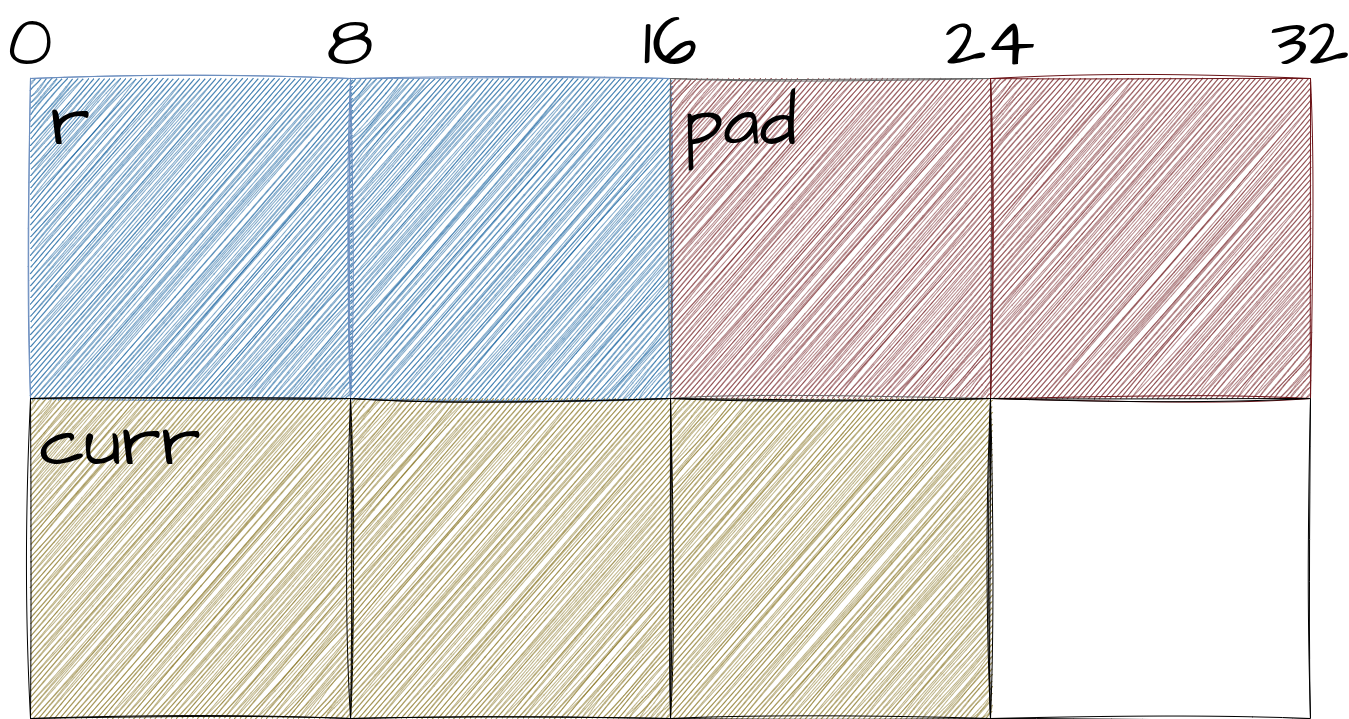
\includegraphics[width=6cm]{./img/address.png}
        \caption[memory]{連続領域への割り当て}
        \label{fig:struct}
      \end{figure}
    \end{column}
  \end{columns}  
\end{frame}
\begin{frame}
  \frametitle{interior pointer(フィールドの内部を指すポインタ)}
  {\large interior pointerを使う間、構造体全体がメモリに残る}
  \begin{figure}[h]
    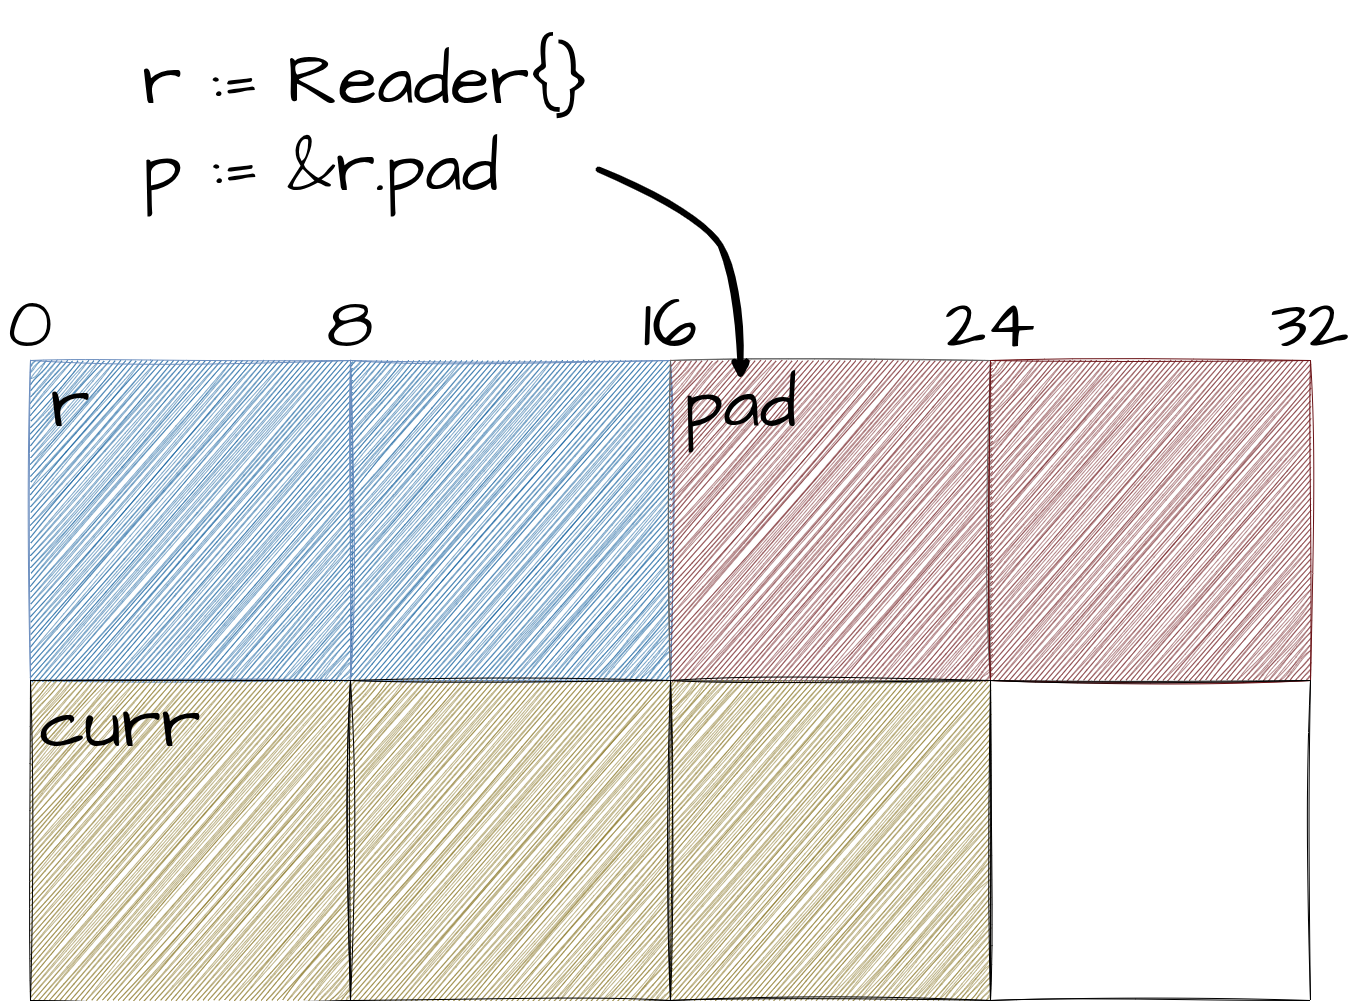
\includegraphics[width=6cm]{./img/interior.png}
    \caption[memory]{interior pointer}
    \label{fig:interor}
  \end{figure}  
\end{frame}
\section{On-the-Fly Garbage Collection}
\begin{frame}
  \frametitle{有向グラフによるヒープの表現}
  {\large ルートから到達できないノードをガベージとみなす}
  \begin{itemize}
  \item 大域やスタックの変数が参照する値はルート
  \item ガベージノードを白に着色
  \item ルートから到達できる中間ノードや葉を黒に着色
  \item ノード数は固定
  \end{itemize}
\end{frame}
\begin{frame}
  \frametitle{灰色がある理由}
  {\large 黒から白に向かう辺がないことを保証したい}
  \par
  \begin{figure}[h]
    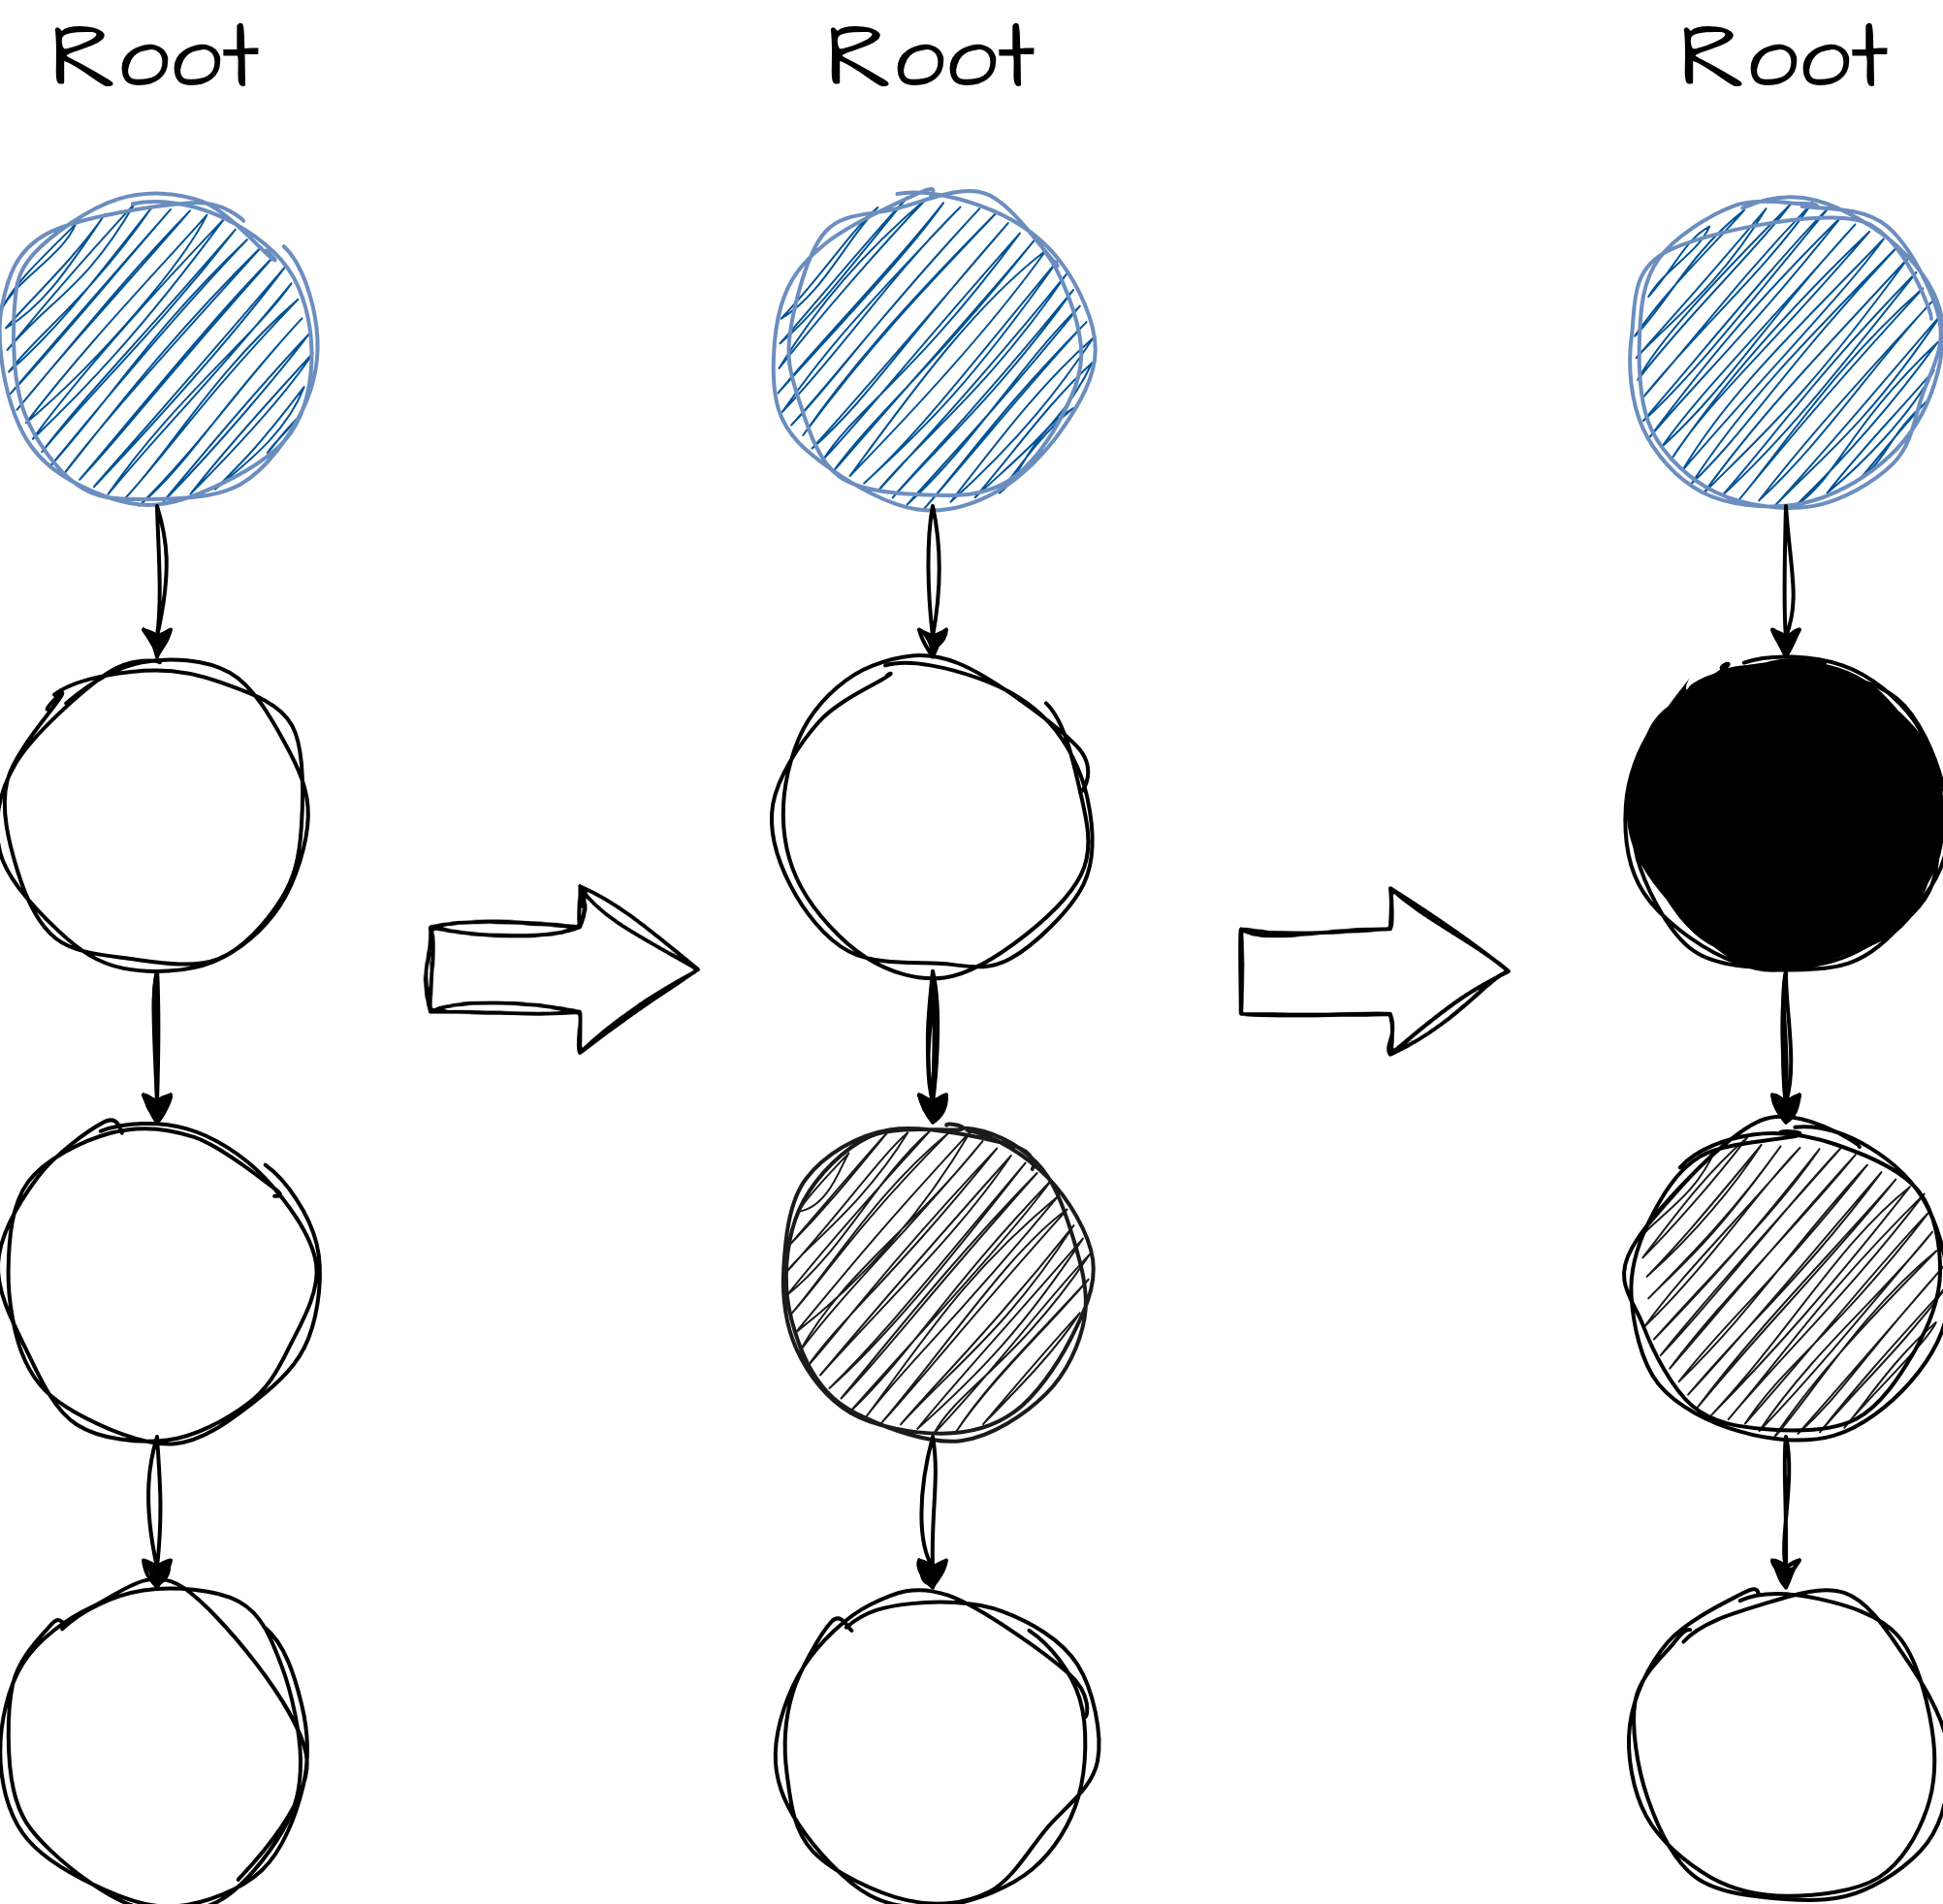
\includegraphics[width=4.8cm]{./img/black-white.png}
    \caption[memory]{黒ノードから白ノードへの参照}
    \label{fig:black-white}
  \end{figure}
\end{frame}
\begin{frame}
  \frametitle{証明の単純化}
  {\large 操作の種類を減らしたい}
  \par
  \vspace{12pt}
  \textcolor{highlight}{操作を多様にするもの}
  \begin{itemize}
  \item ノードが到達できるか
  \item ノードの出次数
  \item 操作の種類: 追加、削除、向き先の変更
  \end{itemize}
\end{frame}
\begin{frame}
  \frametitle{出次数を統一}
  {\large 終端ノード\texttt{NIL}でノードの出次数を2に限定}
  \begin{figure}[h]
    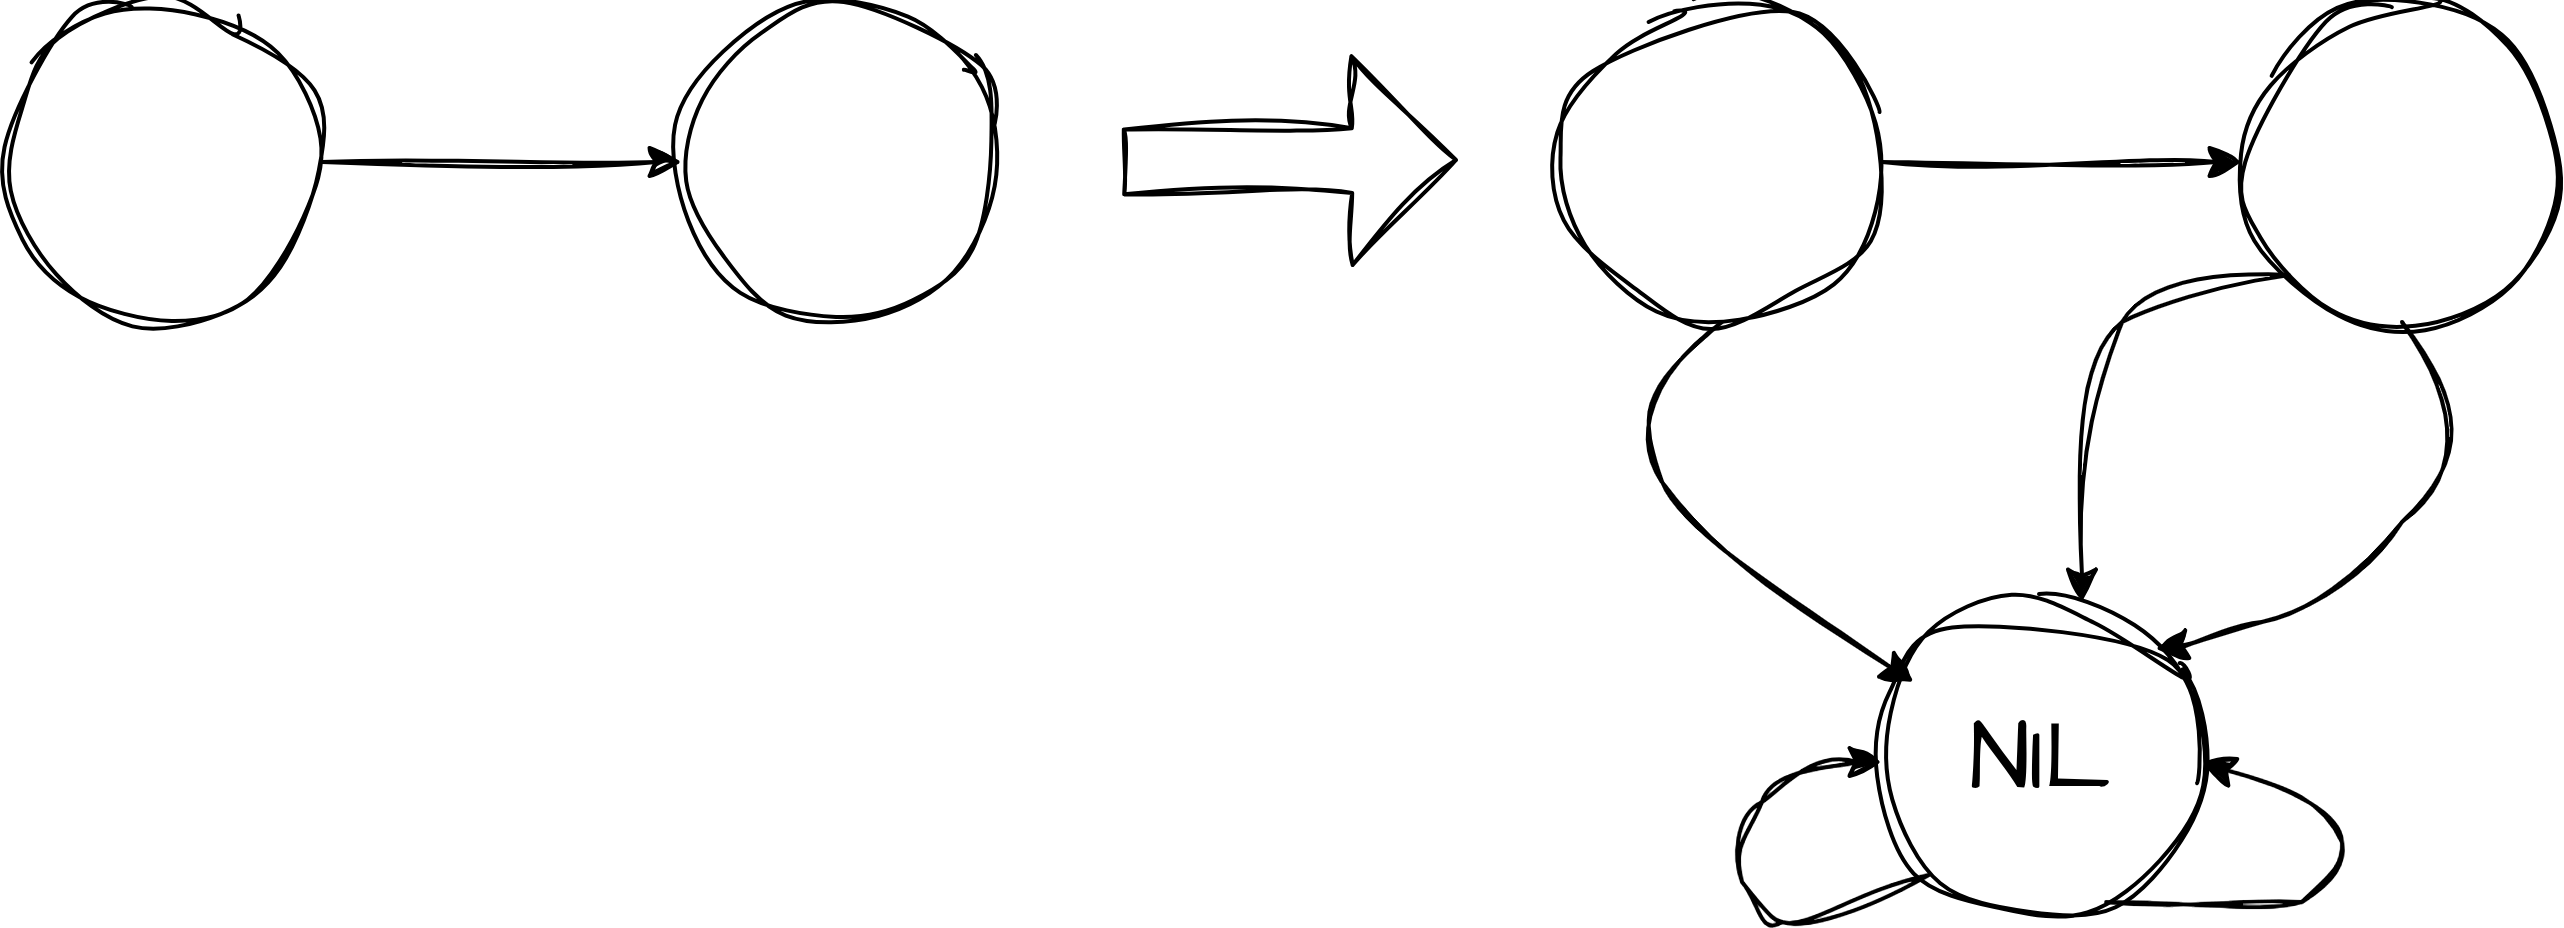
\includegraphics[width=8cm]{./img/nil.png}
    \caption[memory]{\texttt{NIL}の導入}
    \label{fig:nil}
  \end{figure}  
\end{frame}
\begin{frame}
  \frametitle{すべてのノードに到達可能}
  {\large ルートノードでガベージノードのリストをつくる}
  \begin{figure}[h]
    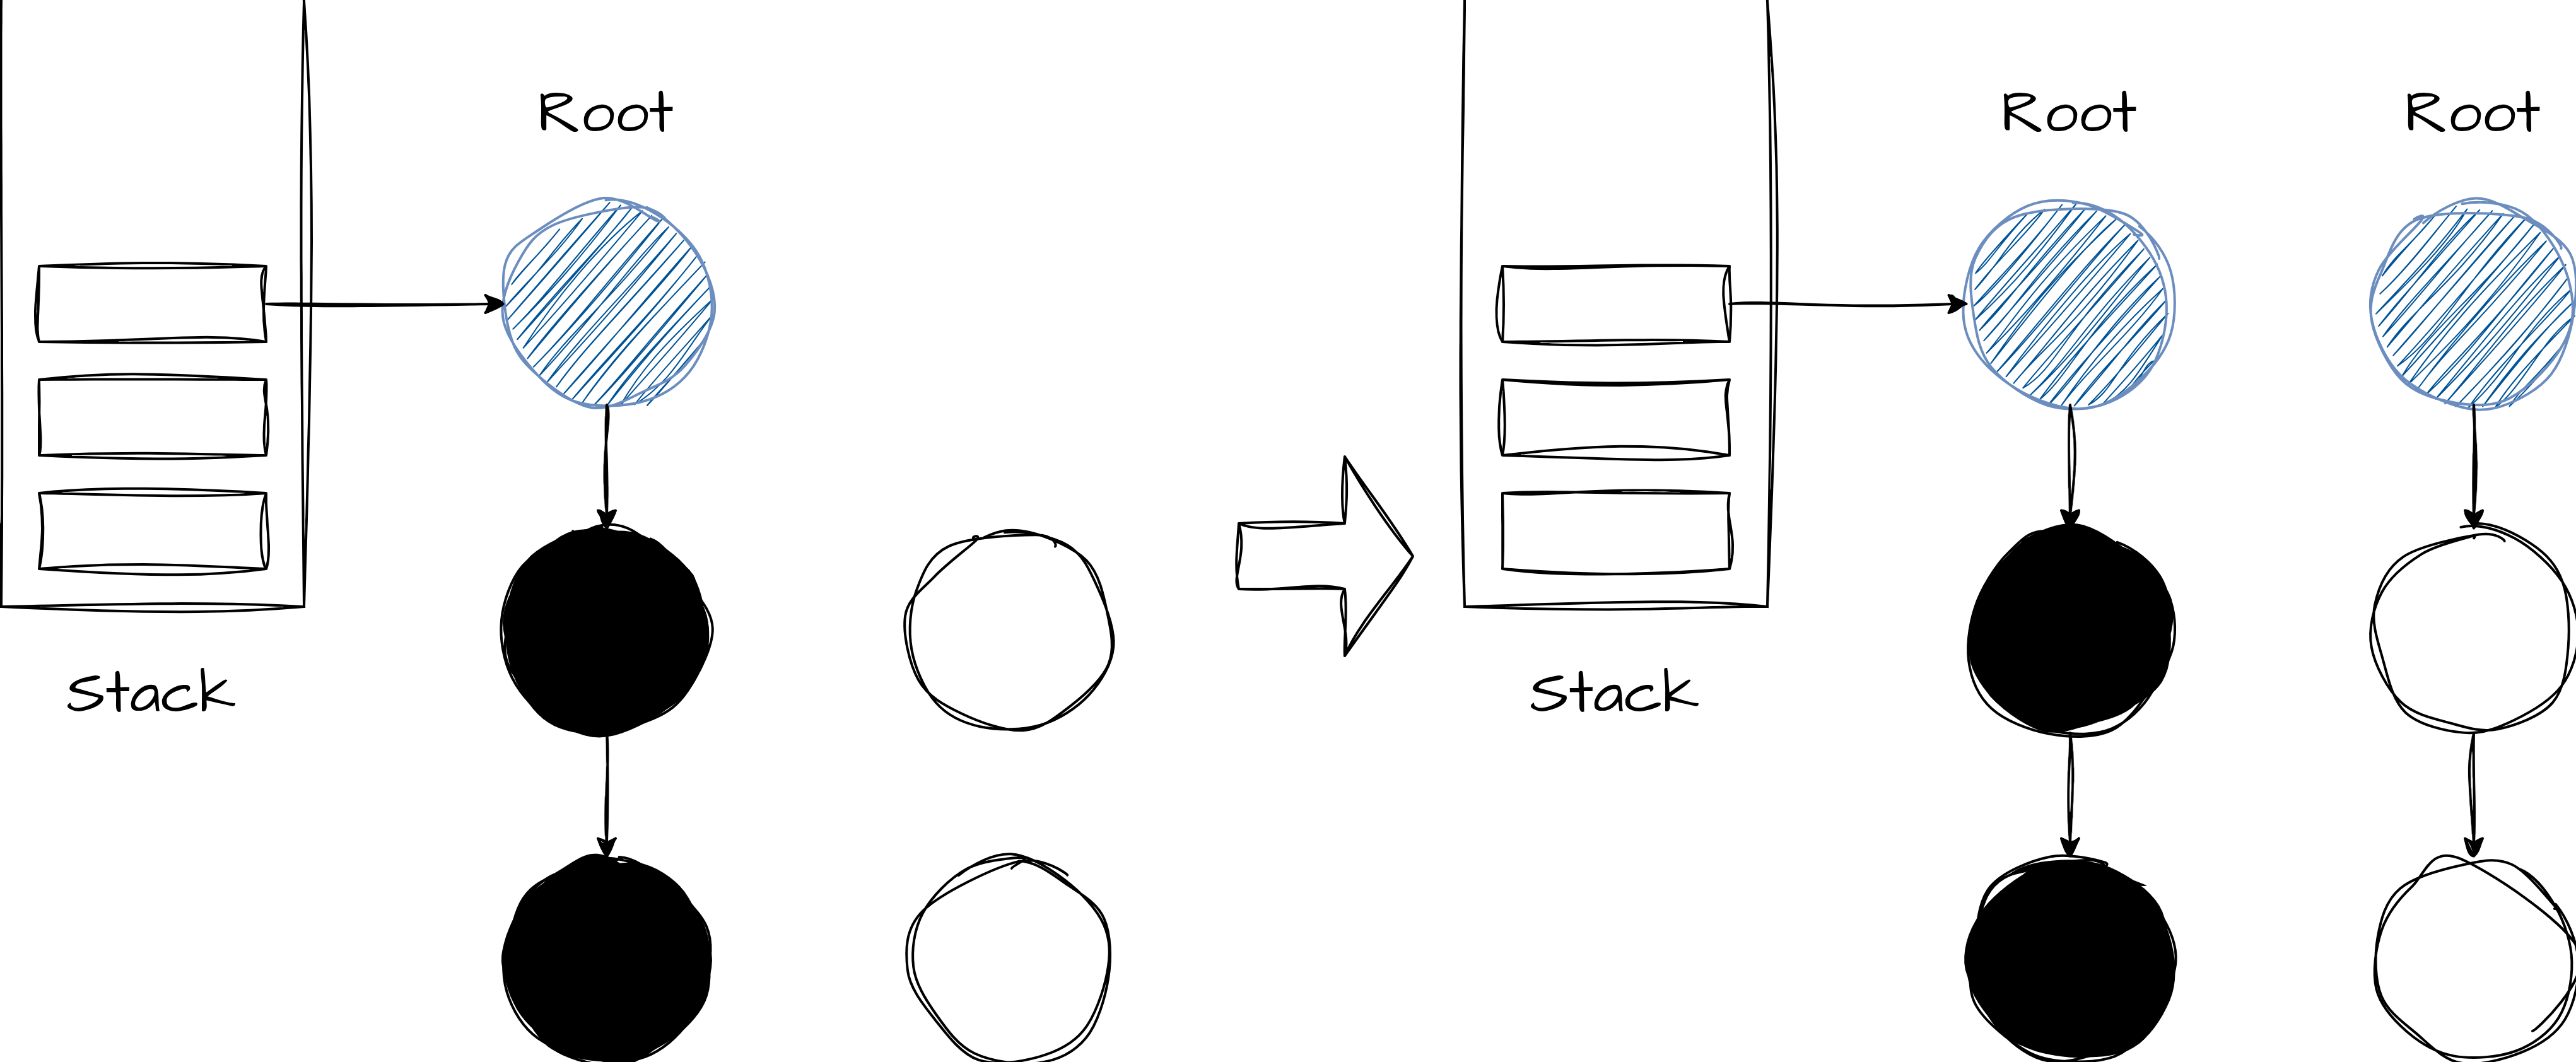
\includegraphics[width=10cm]{./img/freelist.png}
    \caption{リストの導入}
    \label{fig:freelist}
  \end{figure}
\end{frame}
\begin{frame}
  \frametitle{アプリケーション (mutator) の振る舞い}
  {\large 向き先の白いノードを灰にして、辺の向き先を変える}
  \begin{figure}[h]
    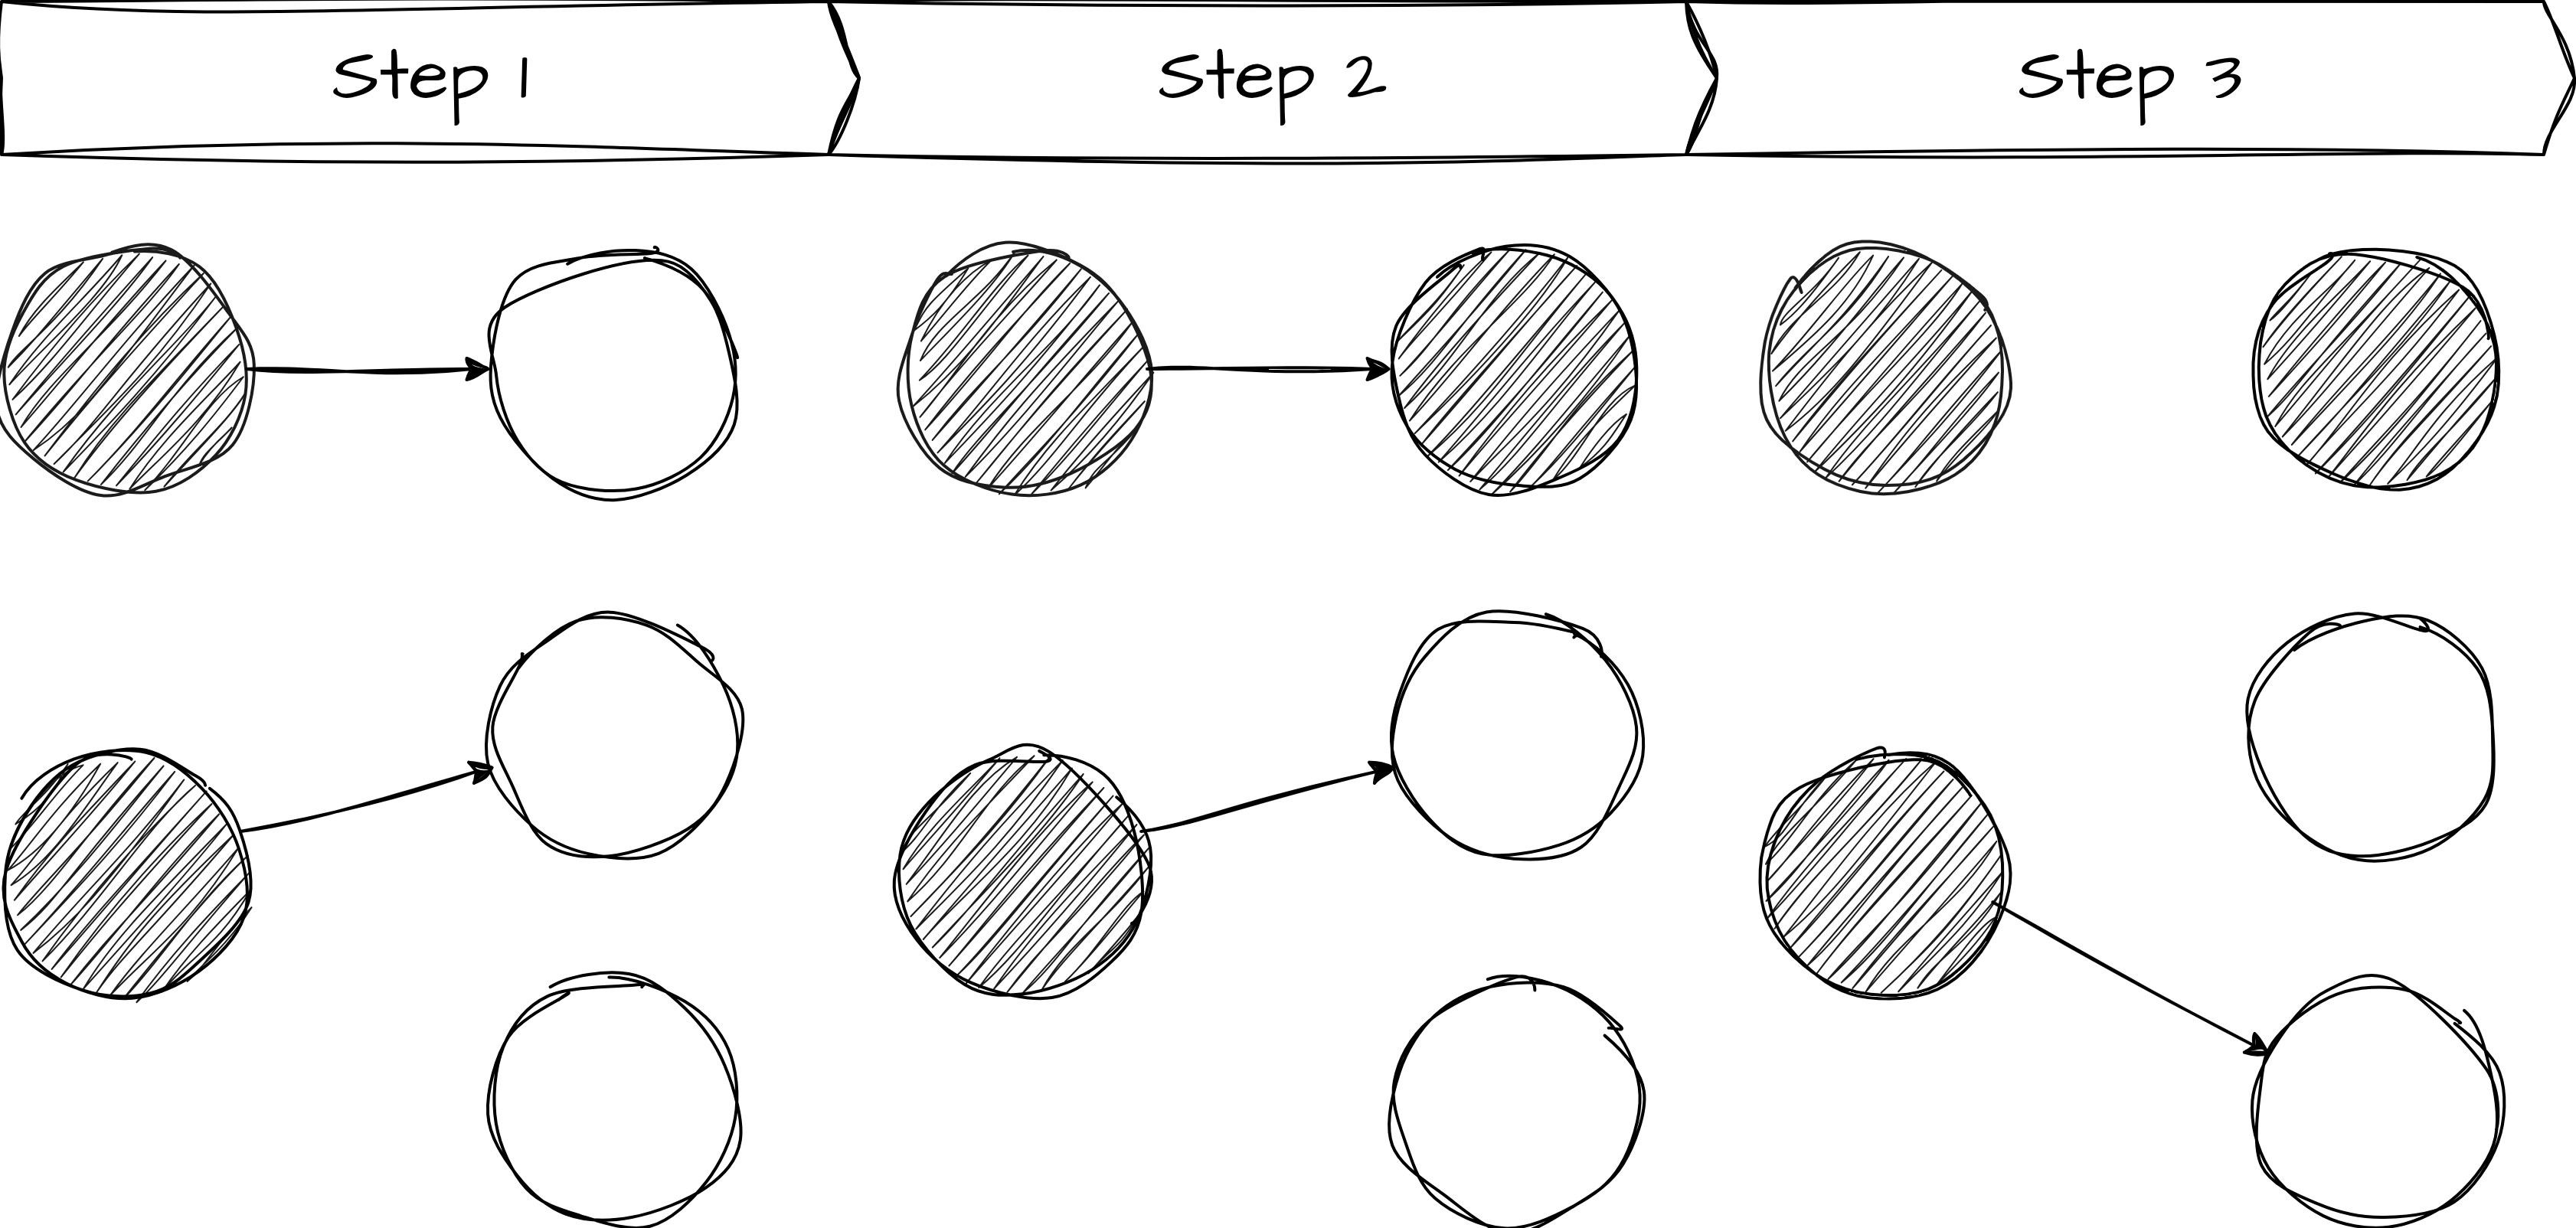
\includegraphics[width=6cm]{./img/mutator.png}
    \caption{mutatorの操作}
    \label{fig:mutator}
  \end{figure}
  \vspace{-1cm}
  \begin{itemize}
  \item step2で、前回変更した有向辺の白い向き先を灰色にする
  \item 向き先が灰か黒ならstep2はいらない
  \item step2とstep3は別のアトミックな操作でいい
  \end{itemize}
\end{frame}
\begin{frame}
  \frametitle{マーキングフェース}
  {\large 後続の白いノードを灰色にして、ノードを黒くする}
  \begin{figure}[h]
    
\includegraphics[width=12cm]{./img/marking.png}
    % \caption{マーキング}
    \label{fig:marking}
  \end{figure}
\end{frame}
\begin{frame}
  \frametitle{マーキングフェースの疑似コード}
  {\large ルートノードを灰色にする}
  \lstinputlisting[language=python,style=pystyle]{./code/marking1.py}
\end{frame}
\begin{frame}
  \frametitle{マーキングフェースの疑似コード}
  {\large 一巡しても灰色ノードがなければ終了}
  \lstinputlisting[language=python,style=pystyle,basicstyle=\scriptsize]{./code/marking2.py}
\end{frame}
\begin{frame}
  \frametitle{アペンディングフェーズ}
  {\large 白ノードをリストに追加し、黒ノードを白にする}
  \lstinputlisting[language=python,style=pystyle]{./code/appending.py}  
  このフェーズには、灰色のノードはない
\end{frame}
\section{ガベージコレクションの実装}
\begin{frame}
  \frametitle{Goのガベージコレクションのフェーズ}
  {\large マーキングの終了時にSTWがある\supercite{go-gc}}
  \begin{figure}[h]
    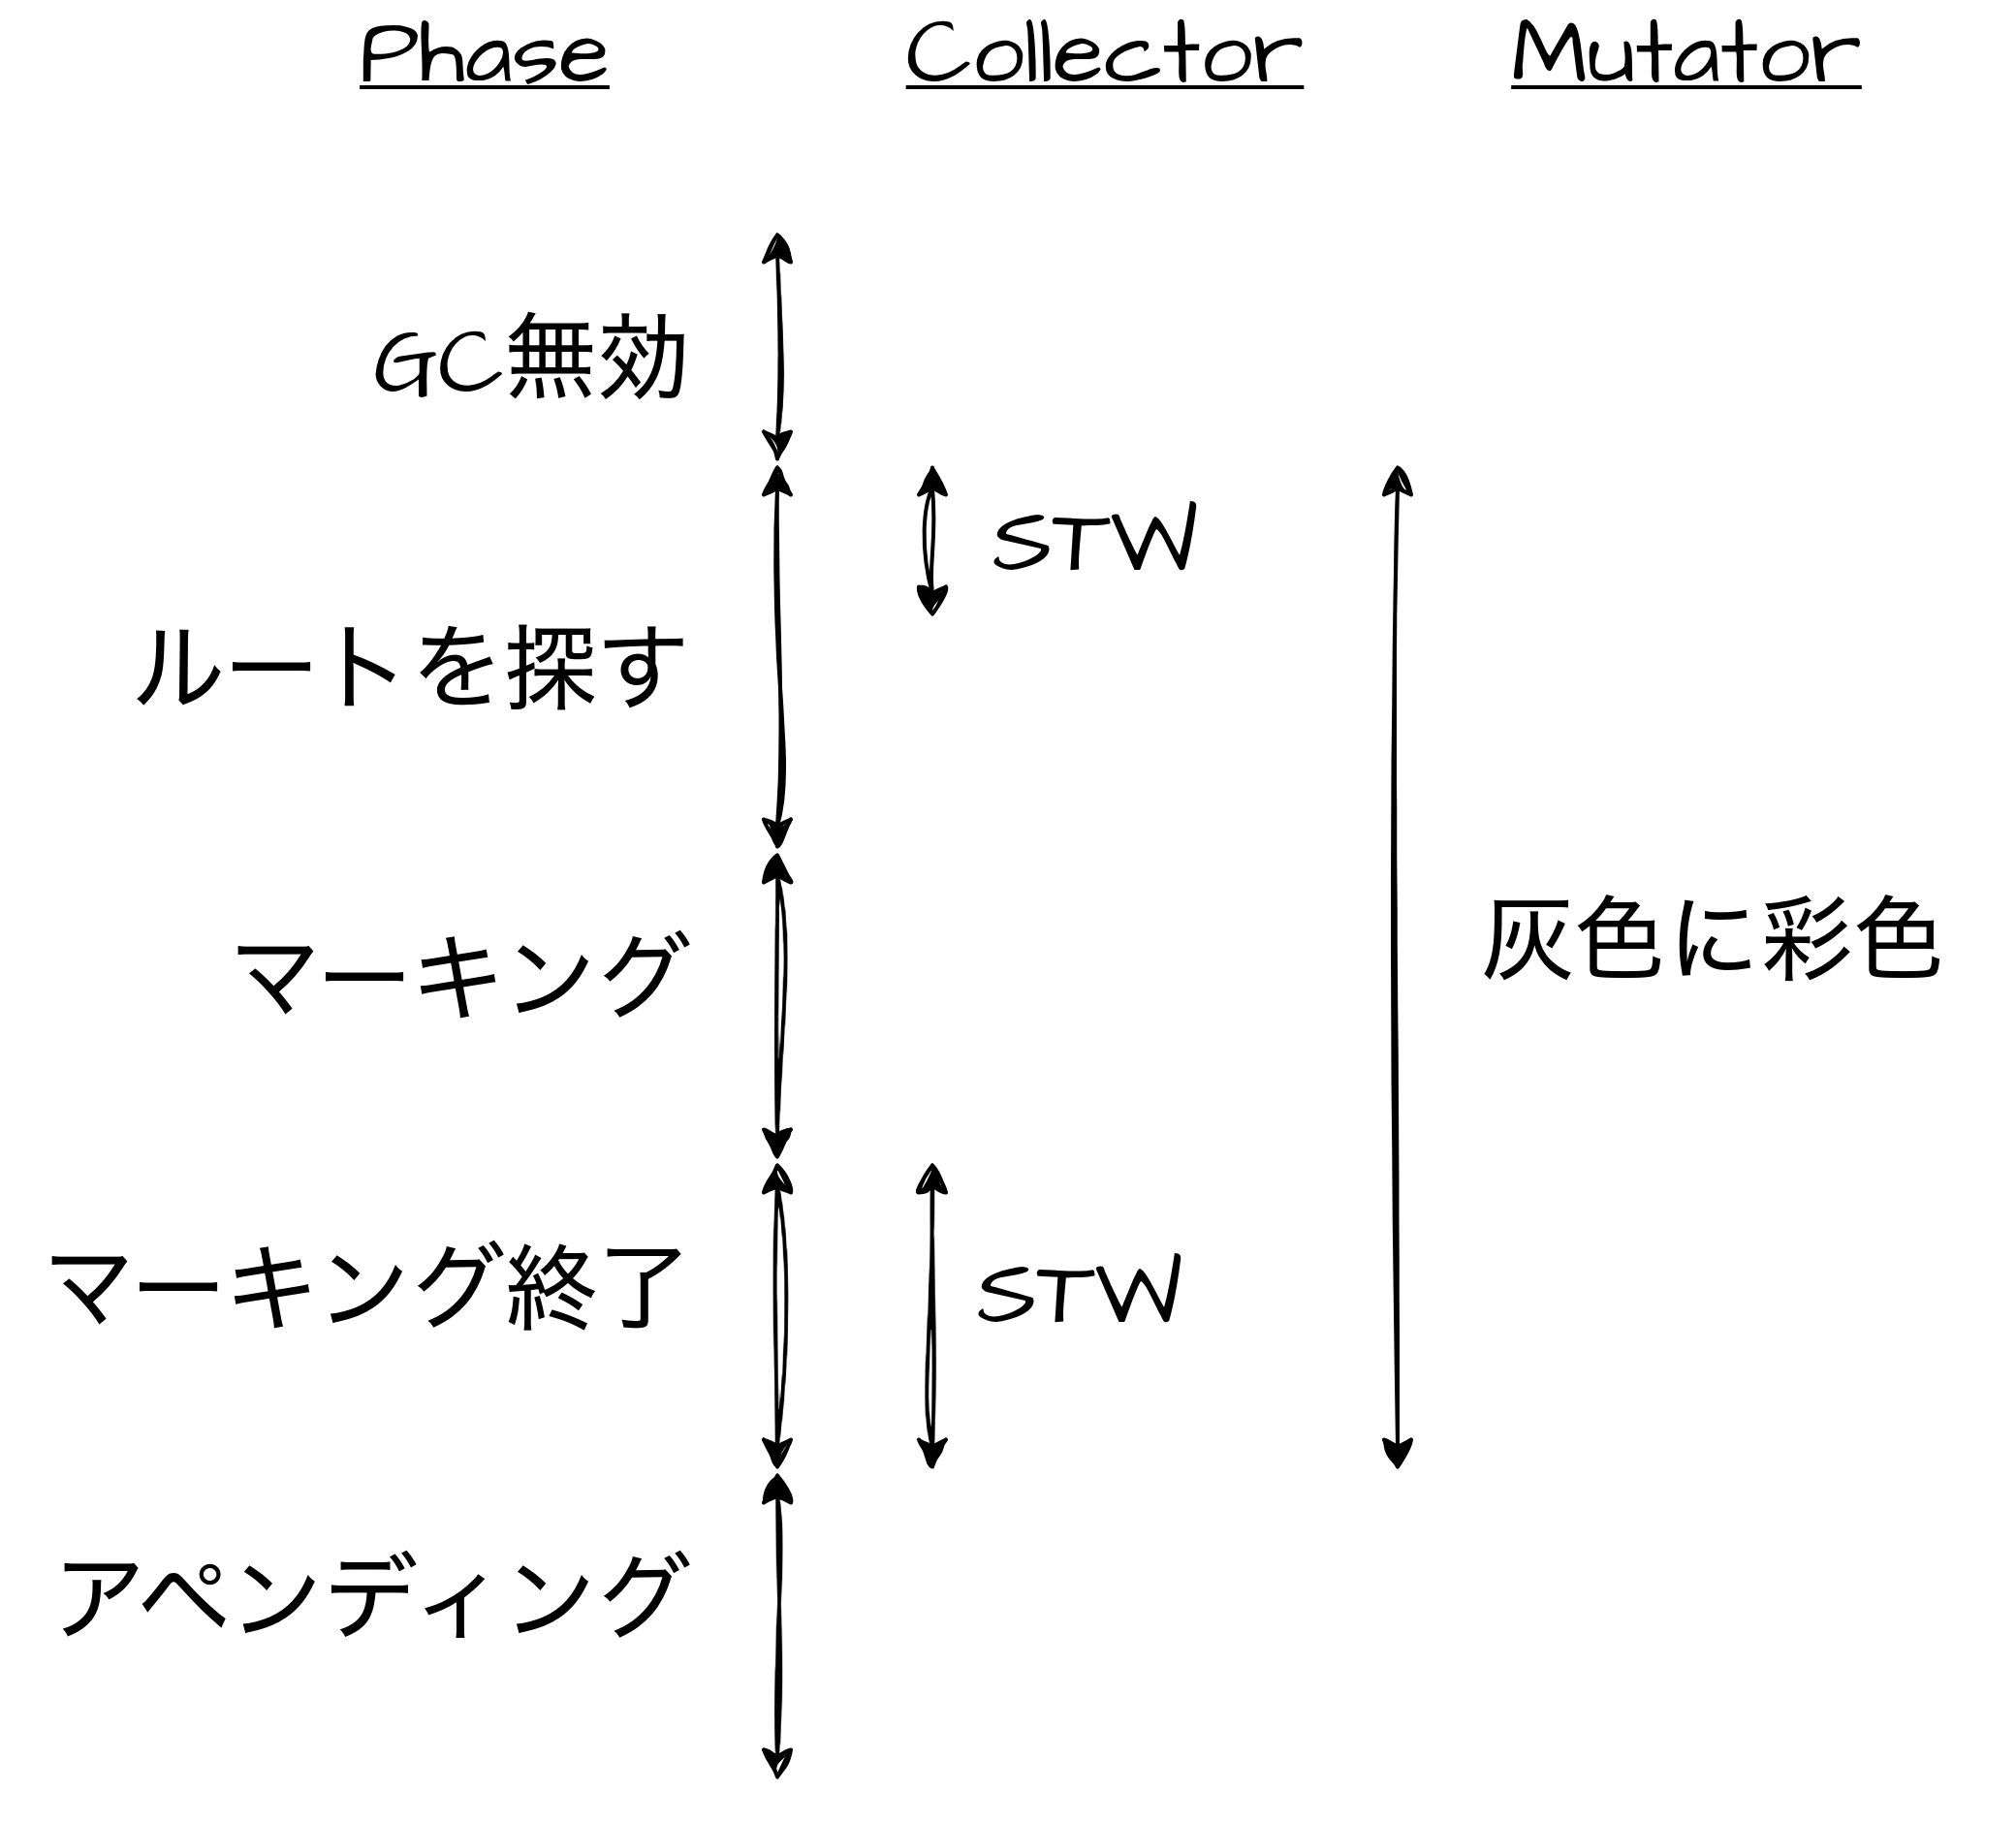
\includegraphics[width=5cm]{./img/phase.png}
    \caption{GoのGCのライフサイクル}
    \label{fig:phase}
  \end{figure}
\end{frame}
\begin{frame}[allowframebreaks,t]
  \frametitle{参考資料}
  \printbibliography
  \nocite{*}
\end{frame}
\end{document}
